\documentclass{article}

\usepackage{fancyhdr}
\usepackage{extramarks}
\usepackage{amsmath}
\usepackage{amsthm}
\usepackage{amsfonts}
\usepackage{tikz}
\usepackage[plain]{algorithm}
\usepackage{algpseudocode}
\usepackage{graphicx}
\usepackage{float}
\usepackage{listings}
\usepackage{xcolor}

\usetikzlibrary{automata,positioning}

%
% Basic Document Settings
%

\topmargin=-0.45in
\evensidemargin=0in
\oddsidemargin=0in
\textwidth=6.5in
\textheight=9.0in
\headsep=0.25in

\linespread{1.1}

\pagestyle{fancy}
\lhead{\hmwkHeaderName}
\chead{\hmwkClass\: \hmwkTitle}
\rhead{\firstxmark}
\lfoot{\lastxmark}
\cfoot{\thepage}

\renewcommand\headrulewidth{0.4pt}
\renewcommand\footrulewidth{0.4pt}

\setlength\parindent{0pt}

\lstset{
    basicstyle=\ttfamily\small,
    breaklines=true,
    frame=single,
    showstringspaces=false,
    numbers=left,
    numberstyle=\tiny,
    keywordstyle=\color{blue},
    commentstyle=\color{gray},
    stringstyle=\color{red}
}


%
% Create Problem Sections
%

\newcommand{\enterProblemHeader}[1]{
    \nobreak\extramarks{}{Task \arabic{#1} continued on next page\ldots}\nobreak{}
    \nobreak\extramarks{Task \arabic{#1} (continued)}{Task \arabic{#1} continued on next page\ldots}\nobreak{}
}

\newcommand{\exitProblemHeader}[1]{
    \nobreak\extramarks{Task \arabic{#1} (continued)}{Task \arabic{#1} continued on next page\ldots}\nobreak{}
    \stepcounter{#1}
    \nobreak\extramarks{Task \arabic{#1}}{}\nobreak{}
}

\setcounter{secnumdepth}{0}
\newcounter{partCounter}
\newcounter{homeworkProblemCounter}
\setcounter{homeworkProblemCounter}{1}
\nobreak\extramarks{Task \arabic{homeworkProblemCounter}}{}\nobreak{}

%
% Homework Problem Environment
%
% This environment takes an optional argument. When given, it will adjust the
% problem counter. This is useful for when the problems given for your
% assignment aren't sequential. See the last 3 problems of this template for an
% example.
%
\newenvironment{homeworkProblem}[1][-1]{
    \ifnum#1>0
        \setcounter{homeworkProblemCounter}{#1}
    \fi
    \section{Task \arabic{homeworkProblemCounter}}
    \setcounter{partCounter}{1}
    \enterProblemHeader{homeworkProblemCounter}
}{
    \exitProblemHeader{homeworkProblemCounter}
}

%
% Homework Details
%   - Title
%   - Due date
%   - Class
%   - Section/Time
%   - Instructor
%   - Author
%

\newcommand{\hmwkTitle}{Assignment 1}
\newcommand{\hmwkDueDate}{Due: 25.03.2026}
\newcommand{\hmwkClass}{Network Modeling}
\newcommand{\hmwkClassTime}{}
\newcommand{\hmwkClassInstructor}{}
\newcommand{\hmwkAuthorName}{\textbf{Group 30:}\\Tristan Gabl, Hristo Georgiev,\\Kevin Halter, Jakob Teetz}
\newcommand{\hmwkHeaderName}{Group 30}

%
% Title Page
%

\title{
    \vspace{2in}
    \textmd{\textbf{\hmwkClass:\ \hmwkTitle}}\\
    \normalsize\vspace{0.1in}\small{Due\ on\ \hmwkDueDate}\\
    \vspace{0.1in}\large{\textit{\hmwkClassInstructor\ \hmwkClassTime}}
    \vspace{3in}
}

\author{\hmwkAuthorName}
\date{}

\renewcommand{\part}[1]{\textbf{\large Part \Alph{partCounter}}\stepcounter{partCounter}\\}

%
% Various Helper Commands
%

% Useful for algorithms
\newcommand{\alg}[1]{\textsc{\bfseries \footnotesize #1}}

% For derivatives
\newcommand{\deriv}[1]{\frac{\mathrm{d}}{\mathrm{d}x} (#1)}

% For partial derivatives
\newcommand{\pderiv}[2]{\frac{\partial}{\partial #1} (#2)}

% Integral dx
\newcommand{\dx}{\mathrm{d}x}

% Alias for the Solution section header
\newcommand{\solution}{\textbf{\large Solution}}

% Probability commands: Expectation, Variance, Covariance, Bias
\newcommand{\E}{\mathrm{E}}
\newcommand{\Var}{\mathrm{Var}}
\newcommand{\Cov}{\mathrm{Cov}}
\newcommand{\Bias}{\mathrm{Bias}}

\begin{document}

\maketitle

\pagebreak

\begin{homeworkProblem}
\begin{enumerate}
    \item[(1)]

    The total number of possible directed ties is
    \[
        n(n-1) = 462.
    \]
    Therefore, the probability of observing a directed tie is
    \[
        p = \frac{134}{462} = 0.2900.
    \]

    \item[(2)]

    As there are 231 dyads, the probabilities are
    \[
        p_M = \frac{42}{231} = 0.1818,
        \qquad
        p_A = \frac{50}{231} = 0.2165,
        \qquad
        p_N = \frac{139}{231} = 0.6017.
    \]

    \item[(3)]

    With tie independence, each directed tie is present with probability \(p\). so,
    \[
        p_M^{\mathrm{ind}} = p^2 = 0.0841,
    \]
    \[
        p_A^{\mathrm{ind}} = 2p(1-p) = 0.4118,
    \]
    \[
        p_N^{\mathrm{ind}} = (1-p)^2 = 0.5040.
    \]

    \item[(4)]

    Assuming independence of ties does not hold up in this case, since the calculated probabilities differ significantly from the observed ones. Mutual and null dyads occur more often than expected, while asymmetric dyads occur less often. Reciprocal ties seem to be much more common than would be expected under an independent process.
    
    \item[(5)]

    If each pupil is assumed to have exactly \(9\) outgoing ties, then the probability of a directed tie is
    \[
        p = \frac{9}{21} = 0.4286.
    \]
    This gives
    \[
        p_M^{\mathrm{ind}} = p^2 = \left(\frac{9}{21}\right)^2 = 0.1837.
    \]
    Compared to the random chance independent $p^{ind}_M$ we get a very close estimate of $p_M$ with our assumption of 9 outgoing edges. The model is very reasonable since pupils might be friends with on average 9 other pupils, although this would probably not be uniformly distributed.
    
    \item[(6)]

    For \texttt{cguRec}, the hypothesis is that the observed reciprocity is higher than expected by chance, with the number of edges fixed. Since \(\Pr(X \geq \mathrm{Obs}) = 0\), none of the random graphs had a reciprocity as high as the observed one \(0.7737\). This strongly suggests that friendships are much more often mutual than one-sided.
    
    For \texttt{cugInd}, the hypothesis is that the observed indegree centralization is higher than expected by chance, again with the number of edges fixed. Since \(\Pr(X \geq \mathrm{Obs}) = 0.7712\), the observed value \((0.2022)\) is not unusually high. This suggests that there is no single pupil or small group of pupils that is much more popular than expected by chance.
    
    For \texttt{cugTrans}, the hypothesis is that the observed transitivity is higher than expected by chance, with the dyad census fixed. Since \(\Pr(X \geq \mathrm{Obs}) = 0\), none of the random graphs had a transitivity as high as the observed one \((0.5360)\). This strongly suggests that pupils tend to be friends with the friends of their friends.
    
    Overall, the network shows clearly higher reciprocity and transitivity than expected by chance, while indegree centralization is not unusually high.
\end{enumerate}

\end{homeworkProblem}

\pagebreak

\begin{homeworkProblem}
\begin{enumerate}
    \item[(2.1)]

    The QAP gives a coefficient of \(0.9998\). This implies a very strong positive association between the friendship network at wave 1 and the friendship network at wave 2. The corresponding p-value is \(0.0\), showing, that the result is also very significant.

    \item[(2.2)]

    We added three dyadic covariate matrices based on the attribute data.

    First, we used the literacy score of the receiver. For this, the literacy value of each student was copied into the corresponding column of the matrix, so that the receiver's literacy score can affect the probability of receiving a friendship tie.

    Second, we created a same-gender matrix. Its entries are \(1\) if two students have the same gender and \(0\) otherwise.

    Third, we used the HISEI value of the sender. For this, the HISEI value of each student was copied into the corresponding row of the matrix, so that the sender's HISEI can affect the probability of sending a friendship tie.

    \item[(2.3)]

    \textbf{Hypothesis i:}\\ The coefficient is negative, but very small and not statistically significant. So there is no meaningful support for the hypothesis.

    \textbf{Hypothesis ii:}\\ The coefficient is negative and statistically significant. So this hypothesis is supported.

    \textbf{Hypothesis iii:}\\ The coefficient is negative and not statistically significant. So there is no support for the hypothesis.

    \item[(2.4)]

    See code.

    \item[(2.5)]

    See table for the estimated values.

    \textbf{Hypothesis i:} The coefficients are all very close to zero and can be either positive or negative. This shows no support for the hypothesis that students with high literacy scores receive fewer nominations.

    \textbf{Hypothesis ii:} The coefficients are mostly small, with both positive and negative values. This suggests that same-gender friendships may be more likely in some classrooms, but the effect is not consistent across all classrooms.

    \textbf{Hypothesis iii:} The coefficients are again very small and can be positive or negative. This shows no evidence that students with higher HISEI scores send more friendship nominations.

    \begin{figure}[H]
        \centering
        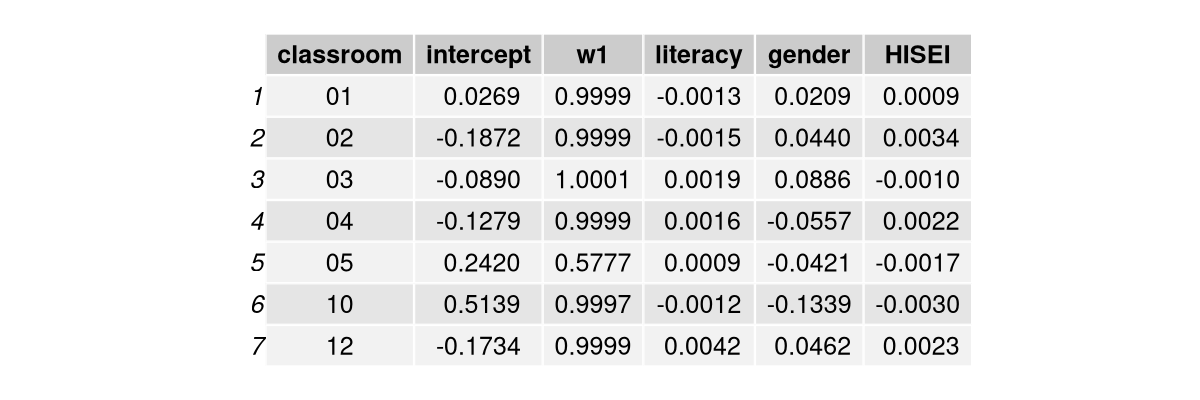
\includegraphics[width=\textwidth]{task2_table.png}
        \caption{QAP coefficients across classrooms.}
    \end{figure}
        
\end{enumerate}
\end{homeworkProblem}

\begin{homeworkProblem}
\begin{enumerate}
    \item[(3.1)] 
    
    See code.

    \item[(3.2)] 
    
    See code.

    \item[(3.3)]
    
    In the NAM model for class 10 wave 2, the network autocorrelation parameter ($\rho_1$) was estimated at $0.613$ and is highly statistically significant ($p < 0.001$). Thus, the data strongly supports the hypothesis that a student's ending literacy score is positively associated with the literacy scores of their friends. 

    Furthermore, when controlling for these network effects, the exogenous variables gender ($p = 0.199$) and socioeconomic status/HISEI ($p = 0.902$) were not statistically significant predictors of a student's ending literacy score.

    
    \item[(3.4)]
    
    With the comparison between MR-QAP and NAM, we can observe the difference between social ties and individual outcomes.
    In MR-QAP, gender homophily was highly significant predictor for friendship ties ($p < 0.001$). Thus, students 
    tended to form same-gender groups. However, in NAM, gender was not statistically significant for predicting the student's ending literacy score.
    
    When it comes to socioeconomic status, both NAM and MR-QAP didn't display statistical significance: HISEI did not affect a student's consideration for 
    friendship ($p = 0.658$), nor did it predict high ending literacy score in NAM ($p = 0.902$).
    
    \item[(3.6)]
    
    Analyzing the network autocorrelation parameter, we see that classrooms 2, 3, 4, 8, 10 and 11 have positive estimates, implying that overall, friendships are correlated with similar literacy scores. However, this cannot be generalized since only classrooms 3, 10 and 11 have strong statistical significance. For the rest of the classrooms, the network effect is not strong enough to be discerned from the random noise. While there is a positive trend, the statistical significance of the autocorrelation hypothesis is not generalizable across all classrooms.
\end{enumerate}
\end{homeworkProblem}

\pagebreak
\section{Code}

\subsection*{task1.R}
\lstinputlisting[language=R]{task1.R}

\subsection*{task2.R}
\lstinputlisting[language=R]{task2.R}

\subsection*{task3.R}
\lstinputlisting[language=R]{task3.R}


\end{document}
